
\chapter{Independent refactored views}

In a project with multiple developers situations may arise where you need to make a change to the structure of the source code that you do not want impact other developers.  Maintaining your own independently ordered view of the source code could be valuable in these circumstances. 

\section{The problem}
% An example of this if you are working on a subproject in which you need to 
% refactor. In some conditions refactoring is only required to simplify the 
% code to implement a small change as opposed to cleaning up the entire code 
% base.  This partial refactoring is likely if the code base is large. 
% According to Melina et. al. \cite{Milea2014} refactoring is a challenge when 
% the code base is large. By definition refactoring does not any functionality 
% but changes the source code. This means that the code previous to being 
% partially refactored is equivalent to the code after the partial 
% refactoring.

% as Refactoring does not change it other programmers could needlessly be 
% impacted by the refactoring changes.. If

% 
% There are other reasons for having a view that is independently
% 

Imagine a situation where you are working jointly on a project with other people. Since you want to collaborate on different aspects of the same source code you have set up the project in a merge based version control system.  You have checked out your own copy of the code so that you can work on the source code without interfering with any of the changes others are making. You notice that you they are going to have to refactor the code before you add any of your changes.  This would be a fair judgement call as Fowler claims that the main time to do refactoring is before making any changes \cite{Fowler1999}. You complete your changes and check in your code back into the version control system.  While you are doing this other people have been working on the code.  If you manage to check in your code before anyone else you will not need to merge any of your changes.  Anybody who checks in after you however, could have a merge conflict.  Some conflicts that they experience could be because the changes you made directly compete with the changes you have made. Potentially more conflicts would occur between the changes they have made and the refactoring that you have completed. This is because a refactoring often makes a large amount of global changes to the source code.

\begin{figure}
\begin{center}
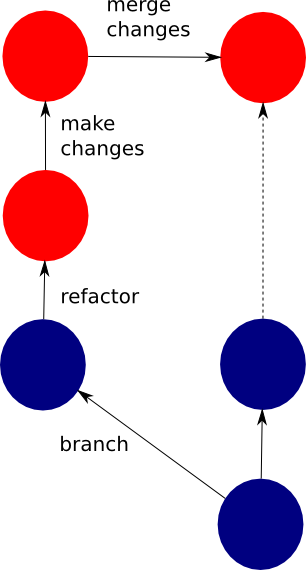
\includegraphics[scale=0.5]{refactorCheckIn}
\end{center}
\caption{Merging changes with refactored code also merges any refactoring}
\end{figure}

As shown in figure the difficulty lies in the fact that not only the functionality that you have added is checked in but also the changes brought about by refactoring.  These refactored changes have not changed how the program functions but have simplified and tidied the code to make the addition of your changes easier. There are some occasions where you may want to avoid changing other peoples code in such a dramatic fashion.  By checking in your refactoring code however, you are forcing others to comply with your vision about how the code should be structured.  This occurs even though you could have no awareness about what changes to the code others have made or intend to make.  Everyone who attempts to check in their code after you will need to merge into a restructured code source that they are unfamiliar with.  This is a recipe for merge based bugs and time wasted doing unnecessary merging.

% Kerievsky also relates a tale about how the lack of knowledge of patterns
% making a particular refactoring look a lot more complex
% \cite{Kerievsky2004}. The different perspectives meant that the programmer
% he refers to as John has a differing opinion that the refactored code was
% not an improvement. This shows that it is not just different functionality
% that influences the need to refactor but sometime the knowledge and
% experience of the developers themselves. It is often the case that two
% developers could have different views about what is an appropriate
% refactoring. This could be because each person brings different skills,
% notices different issues and has a preferred way of visualizing a problem
% and solution.
% 

% 
% then created a branch
% If they attempt to check-in their changes there is the possibility a
% conflict with any of your changes.
% 
% You also need to refactor the code to do your work but both of the
% refactorings are different because they clarify or highlight different
% aspects of the source code.
% 
% If there is some refactoring before any changes are made when the code is
% merged with the original project (often called the trunk project) both
% the changes and the refactored code are checked in.






When there is a large change on a separate branch it could be the case that there are multiple check-ins to keep other parts up to date and ensure that there is not too much divergence.  Currently if you have a project where there are periodic check-ins for each development milestone there will be a large impact each time there is a commit. This is because the refactoring for the large refactored project is imposed upon the repository each time it is checked in.

One of the ways this can be dealt with is by creating separate branches for different projects however this has some issues with merging when working on two or more projects simultaneously.  In order to minimise the amount of divergence it is advisable to merge each of the branches with the trunk often.  If there has been global refactoring changes introduced by one project being merged the merge will be worse for any of the remaining branches when they are checked in.  Instead of having an issue merging at the check-in level we now have an issue at the merging of branches.  As these changes will occur less often than checking in the code, the code will possibly have more divergence.  This divergence is likely to cause more rather than less merge issues at the expense of having to merge less often.


One of these changes which is not catered for by current version control systems is the change of order.  The first person to check-in their code will have no issue as the version control system assumes that all the changes are simply a new revision.  When the second person attempts to reconcile their view there is the possibility of having unnecessary conflicts.  A lot of these conflicts will be with refactored code which although works the same has a different structure.

\section{How we would like to address the problem}
We want to be able to maintain private views or separate branches that can have different but equivalent refactoring.  When these branches are merged we want to make sure that any source code that is equivalent but refactored is not merged to the view we are merging into. Any source code that changes the behaviour however is considered in the merge.

By maintaining two differently refactored view it allows software developers to work on the same programming project to freely refactor with minimal interference to others.
If two software developers refactor the code that they are able to hold their own individual refactoring with reduced changes when they are merged.
The reduced changes would also mean that there will be less unnecessary merge conflicts when merging code.

We also want to be able to further classify more complex operations in a change set than insert, delete and modify.  When JGit compares files with each other because they are structured it can determine if the file has been moved to a different location in the tree.  At this level JGit can also detect copies and renames.  However once JGit starts comparing source code it loses this structural information.  By giving JGit some idea about the structure in the file it can determine these item at the finer granularity of sections of code rather than at a file basis.
